\documentclass[a4paper,10pt]{scrartcl}
\usepackage[utf8]{inputenc}
\usepackage[ngerman]{babel}
\usepackage{amsmath}
\usepackage{amsfonts}
\usepackage{amsthm}
\usepackage{graphicx}
\usepackage{geometry}
\usepackage{multicol}
\geometry{a4paper,left=30mm,right=30mm, top=3cm, bottom=2cm} 

\newcommand{\underfat}[1]{\underline{\textbf{#1}}}
\newcommand{\theuebungszettel}{3}

\parindent0pt

\begin{document}

\begin{center}
  \begin{huge}
    \underfat{Fortgeschrittene funktionale}\\
    \underfat{Programmierung in Haskell}\\
  \end{huge}
\begin{LARGE}
\textbf{Übungszettel \theuebungszettel}

\end{LARGE}
\end{center}

\section*{Aufgabe \theuebungszettel.1:}

Fünf Seemänner stranden auf einer Insel, deren einziger anderer Bewohner ein Affe ist. Um ihr Überleben zu sichern sammeln sie am ersten Tag $n$ Kokosnüsse auf Vorrat. \smallskip

In der Nacht wacht ein Seemann auf und befürchtet, am nächsten Tag nicht seinen fairen Anteil der Nüsse zu bekommen. Also teilt er den Haufen Kokosnüsse in fünf gleiche Teile auf. Dabei bleibt genau eine Kokosnuss übrig, die er dem Affen gibt. Der Seeman versteckt darauf hin sein Fünftel der Nüsse und tut alle verbleibenden wieder auf einen Haufen und legt sich schlafen.\smallskip

Kurz darauf wacht der zweite Seemann auf und auch er fürchtet um seinen Anteil. Er teilt den (jetzt kleineren) Stapel ebenfalls in fünf gleiche Teile, abermals bleibt dabei eine Kokosnuss für den Affen übrig. Er versteckt seinen Teil, tut den Rest wieder auf einen Haufen und legt sich wieder schlafen.\smallskip

Dieser Vorgang passiert mit allen fünf Seemännern. Jedes Mal wird der Stapel kleiner und jedes Mal bleibt eine Kokosnuss für den Affen. Am nächsten Tag wachen alle Seemänner auf und teilen den verbleibenden Haufen gerade durch fünf auf (dieses Mal bleibt nichts für den Affen). Alle merken, dass der Haufen kleiner ist am Vortag, allerdings sagt niemand etwas weil alle wissen, dass sie mitschuld sind.\bigskip

Die Frage ist: Mit welcher Anzahl Kokosnüsse sind die Seemänner gestartet? Schreiben Sie ein \texttt{Haskell}-Programm, dass die (kleinste) Lösung dieses Rätsels berechnet. Verallgemeinern Sie danach, sodass ihr Programm auch den allgemeinen Fall von $k$ Seemännern bearbeiten kann.

\section*{Aufgabe \theuebungszettel.2:}

Stellen Sie sich vor, Sie sind im Dienst der Majestät für den britischen Geheimdienst \texttt{MI6} tätig, werden allerdings auf einer Mission gefangen genommen. Als Sie aufwachen, befinden sich zwischen einer Klippe (zwei Schritte hinter Ihnen) und einem Nest voller giftiger Schlangen mit sehr schlechtem Atem (zwei Schritte vor Ihnen).

Ihr Gegenspieler versichert Ihnen, dass er Sie freilassen wird, wenn sie eine Sequenz von $12$ Instruktionen angeben können, die sie weder in das Schlangennest noch über die Klippe treten lässt (eine einzelne Instruktion ist entweder \glqq ein Schritt nach vorne\grqq\ oder \glqq ein Schritt nach hinten\grqq ). Sie werden jedoch gewarnt, dass sich ihr Gegenspieler, \emph{nachdem} Sie die Sequenz angegeben haben, entscheiden kann, ob Sie die ganze Sequenz ausführen müssen oder nur jede zweite (Instruktionen $2,4,6,\dots$), dritte (Instruktionen $3,6,\dots$), vierte, fünfte oder sechste (nur Instruktionen $6$ und $12$) Instruktion. Ihre Sequenz muss also auch für all diese Fälle geeignet sein. 

\begin{center}
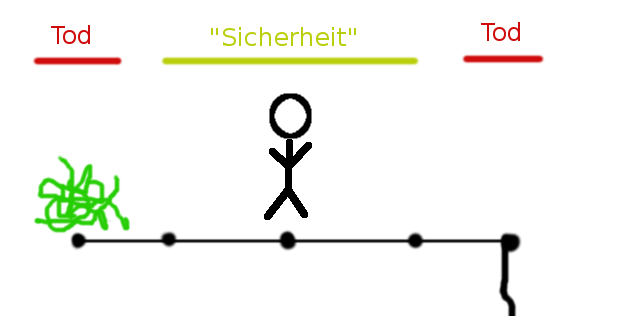
\includegraphics[scale=0.3]{discrepancy.png} 
\end{center}

Finden Sie eine gute Repräsentation des Problems in \texttt{Haskell} und schreiben Sie ein Programm, um herauszufinden, ob es eine Sequenz von $12$ Instruktionen gibt, die Sie auf jeden Fall überleben lässt. Wie sieht es mit $11$ oder $13$ oder $n$ Instruktionen aus?\smallskip

\underline{Hinweis:} Wer mehr über den mathematischen Hintergrund dieses Problems erfahren will, wird schnell unter dem Suchwort \glqq Erdős discrepancy problem\grqq\ fündig.

\end{document}